%======================================================================
\section{Introduction}
\label{sec:introduction}
%======================================================================

Learned surrogates of chaotic partial differential equations usually
compress the whole state into one latent vector and learn how that
vector evolves \citep{linotgraham2022,racca2023,ozalpmagri2025}. For
many systems this is the right design. For spatiotemporally chaotic
systems on large domains it is not, for a reason that is structural
rather than technical. Such systems are extensively chaotic: the number
of active degrees of freedom, measured by the Kaplan--Yorke dimension
$\DKY$, grows in proportion to the domain
\citep{ruelle1982,manneville1985,egolfgreenside1994}. A latent vector
fixed at training time has no size to grow into. A model trained on one
domain cannot even be evaluated on another, and every new domain size
requires new data and new training.

The same structure matters for data assimilation. Ensemble filters in a
global latent space need, without localization, at least as many
members as the attractor has unstable directions
\citep{bocquetcarrassi2017,takeda2026}, a number that grows with the
domain. In physical space the remedy is localization: in extensive chaos
the errors within a region span few directions
\citep{patil2001,ott2004}, so each region can be analysed with a small
ensemble \citep{hunt2007}. A global latent vector has no notion of region
or distance, so this remedy is unavailable, and recent latent filters
either omit localization or leave it for future work
\citep{chen2023roadenkf,tong2026laeenkf}.

We study the alternative: a latent \emph{field}, with a few channels at
each site of a lattice that tiles the physical domain, built only from
operators that are shared by all sites and read a bounded neighbourhood
(Fig.~\ref{fig:concept}).
The parameters of such a model do not depend on the number of sites, so
a model trained at one size is applied to a larger domain by adding
sites, with no retraining. Its latent has a physical geometry, so
localization has a distance to act on. A local, weight-shared model is
also extensive by construction, like the coupled lattice maps whose
Lyapunov spectra have a thermodynamic limit \citep{livi1986,isola1990}
and can be predicted from small subsystems \citep{carretero1999}. The
question is whether a \emph{learned} local rule reproduces the right
density of chaos, and whether it keeps doing so on domains it was never
trained on.

Three things turn out to matter, and they organize the paper. First, the
local rule must be learned from data that contain the statistics of a
large domain: the same architecture trained on a small periodic box
fails under transfer, while trained on windows of one large simulation,
with the window's boundary driven by the simulation, it transfers.
Second, the propagator must stay chaotic when it runs freely: rollouts
that are too short admit spurious regimes, and squared-error rollouts
that are too long damp the dimension. Third, for data assimilation the
locality must survive the decoder: with a decoder that reconstructs each
patch from its own site, the latent observation operator is exactly
local.

No model of a real system is correct, and for many systems of interest
the equations are incomplete or unknown, while observations, with errors
that are usually well characterized, are plentiful. A learned surrogate
that is local can be trained on noisy data of the system itself and used
inside an ensemble filter on any domain; Part~II asks when that is better
than a filter built on imperfect equations.

We hold the models to a demanding standard: their own Lyapunov spectra,
computed from the learned maps, compared with spectra of the true PDE at
every domain size, with the uncertainty of the reference measured rather
than assumed. We do this for the one-dimensional Kuramoto--Sivashinsky
(KS) equation, its two-dimensional isotropic form, and two-dimensional
Kolmogorov flow with linear drag at three drag coefficients.

\begin{figure*}[htbp]
\centering
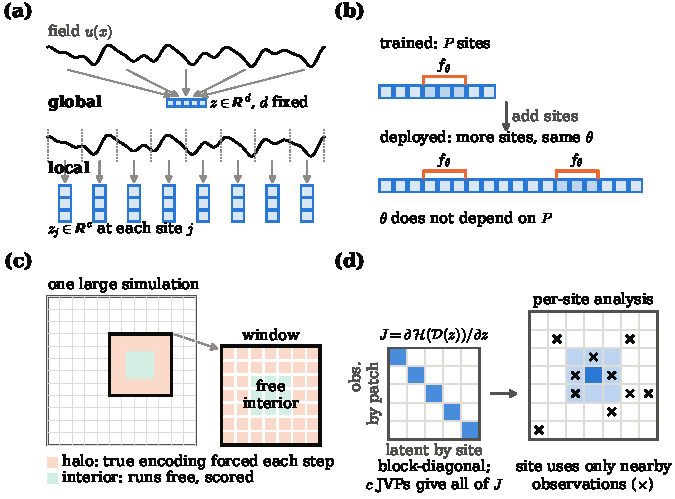
\includegraphics{figures/fig01_concept.pdf}
\caption{The idea in four panels. (a) A global latent compresses the
whole field into one vector of fixed dimension $d$; a local latent field
assigns $c$ channels to the site of each patch. (b) Because every
operator is shared across sites and reads a bounded neighbourhood, the
trained parameters $\theta$ do not depend on the number of sites, and the
model is deployed on a larger domain by adding sites. (c) Training on
windows of one large simulation: at every step of a training rollout the
halo of the window is overwritten by the true encoding, the interior
runs free, and only the interior is scored, so the loss is exactly that
of a limited-area model (Proposition~\ref{prop:halo}). (d) With a
per-patch decoder, the Jacobian of the observations with respect to the
latent is block-diagonal, so it is obtained from $c$ forward-mode
derivatives at any domain size and each site can be analysed from nearby
observations alone (Part~II).}
\label{fig:concept}
\end{figure*}

\para{Contributions.}
\begin{itemize}
\item \emph{A local latent field for extensive chaos}
  (Sec.~\ref{sec:method}): weight-shared encoder, decoder and propagator
  of finite reach, exactly translation-equivariant, with a parameter
  count independent of the domain size: about $135{,}000$ parameters describe
  the local law once, and the same parameters run domains of any size.
\item \emph{Zero-shot transfer validated by Lyapunov spectra}
  (Sec.~\ref{sec:results1d}). Trained at $L=100$, a 1D KS model reproduces
  the true $\DKY$ to within $0.2$--$1.2\%$ from $L=50$ to $L=400$, three
  training seeds agree to within $1.2\%$, and the whole positive part of
  its Lyapunov spectrum collapses onto the truth's.
\item \emph{The training distribution decides transfer}
  (Sec.~\ref{sec:results2d}). Trained on a small periodic box, the same
  architecture misses $\DKY$ by $15$--$38\%$ on larger domains in three of
  four cases in two 2D systems, and adding non-local inputs makes this
  worse. Trained on
  windows of one large domain, with the window's boundary driven by the
  simulation, the final models are within $0.6$--$2\%$ of the truth in 2D
  KS and $1$--$9\%$ in Kolmogorov flow at the two stronger drags, and
  within the truth's own uncertainty in their scaling with domain size;
  the weakest drag is harder. The window training is a learned
  limited-area model, and we prove it trains that problem exactly.
\item \emph{What fails, and why} (Sec.~\ref{sec:failure}): softmax
  attention, short rollouts and squared-error damping, with a lemma that
  connects the last to an underestimate of $\DKY$, and a model-selection
  rule that uses no ground truth.
\item \emph{Exactly local latent data assimilation}
  (Sec.~\ref{sec:da_results}). With a per-patch decoder the latent
  observation Jacobian is block-diagonal and is obtained from as many
  forward passes as there are channels, at any domain size, so a per-site
  ensemble filter in latent space is exact. Running it on four copies of the
  patch lattice shifted by half a patch and blending them removes the error
  tied to the lattice and lowers the analysis error by about $30\%$ without
  retraining; the gain comes from the offsets, not from the extra members.
  With one model trained only on noisy fields, and one setting, the analysis
  error is $0.30$--$0.33$ on every domain from $44^2$ to $440^2$, against $0.82$ for
  interpolating the observations, while an unlocalized filter fails once
  the attractor has more unstable directions than the ensemble has members.
\item \emph{Learned versus physics-based filters} (Sec.~\ref{sec:da_model_error}).
  Against a physics-based ensemble filter whose model is wrong, given
  online parameter estimation and bias correction, the latent filter loses
  when the model error is small or correctable and wins when it is large or
  structural. The outcome is predicted by one number, the part of the
  physical model's one-cycle forecast error that bias correction cannot
  remove: the crossover is near a sixth of the observation error.
\end{itemize}

What is not new should be said as clearly. Localized reduced models of KS
were built from wavelets a quarter century ago \citep{wittenberg2001},
learned models of KS have reproduced Lyapunov spectra at a single size
\citep{pathak2017,vlachas2020,ozalpmagri2025}, and convolutional
surrogates have been run on larger domains than they were trained on
\citep{barsinai2019,kochkov2021}. Section~\ref{sec:background} places our
results among these. The contrast with minimal flow units, which are
non-extensive by construction and where a global latent vector works
well \citep{constanteamores2025}, is the one-sentence summary of when a
field-valued latent is needed.

The paper has two parts. Part~I (Secs.~\ref{sec:method}--\ref{sec:results2d}
and \ref{sec:failure}) concerns the dynamics: the model and its
properties, the systems and the precision of their ground truth, transfer
in one and two dimensions, and the failure modes. Part~II
(Sec.~\ref{sec:da_results}) concerns data assimilation. Section~\ref{sec:discussion}
discusses what transfer requires and the limitations of this study.
